\documentclass[a4paper,titlepage]{article}
\usepackage{graphicx}
\usepackage{float}
\usepackage[utf8]{inputenc}
\usepackage{amsmath}
\usepackage[noend]{algorithmic}
\usepackage{color}
\usepackage{floatpag}
\usepackage{listings}
\usepackage{textcomp}
\usepackage{caption}
\usepackage{afterpage}
\usepackage{titling}
\usepackage{titlesec}
\usepackage{pbox}
\usepackage{tabularx}
\linespread{1.3}
\newcommand{\subtitle}[1]{%
  \posttitle{%
    \par\end{center}
    \begin{center}\large#1\end{center}
    \vskip0.5em}%
}
\renewcommand{\lstlistingname}{Code}

\definecolor{listinggray}{gray}{0.9}
\definecolor{lbcolor}{rgb}{0.9,0.9,0.9}
\lstset{
backgroundcolor=\color{lbcolor},
		tabsize=3,
		linewidth=13.5cm,
		language=MATLAB,
        basicstyle=\scriptsize,
        upquote=true,
        aboveskip={1.5\baselineskip},
        columns=fixed,
        showstringspaces=false,
        extendedchars=false,
        breaklines=true,
        prebreak = \raisebox{0ex}[0ex][0ex]{\ensuremath{\hookleftarrow}},
        frame=single,
        numbers=left,
        showtabs=false,
        showspaces=false,
        showstringspaces=false,
        identifierstyle=\ttfamily,
        keywordstyle=\color[rgb]{0,0,1},
        commentstyle=\color[rgb]{0.026,0.112,0.095},
        stringstyle=\color[rgb]{0.627,0.126,0.941},
        numberstyle=\color[rgb]{0.205, 0.142, 0.73}
}
\lstset{
    backgroundcolor=\color{lbcolor},
    tabsize=2,
  language=sh,
  captionpos=b,
  tabsize=3,
  frame=lines,
  numbers=left,
  numberstyle=\tiny,
  numbersep=5pt,
  breaklines=true,
  showstringspaces=false,
  basicstyle=\footnotesize,
%  identifierstyle=\color{magenta},
  keywordstyle=\color[rgb]{0,0,1},
  commentstyle=\color{green},
  stringstyle=\color{red}
  }


\titlespacing*{\subsubsection}{0pt}{1.1\baselineskip}{\baselineskip}

\begin{document}
\pagenumbering{gobble}
%topmatter
\title{Assignment 2 IM - ECG Analysis}
\author{Gerardo Vitagliano - 2017214620 \\ Martin Schlegel - 2017190694 }
\date{\vspace{-5ex}}
\vfill
\maketitle
\clearpage
\section{Introduction}
Following the assignment request, two different systems have been developed: a detector for a PVC and a detector for Atrial Fibrillation occurencies. These two classifiers take as input the ECG data from a patient, extract the relevant features such as the R peaks, and output a binary value that reflects whether the events have occured or not.\\
The performances of the systems will be compared using sensitivity and specificity parameters.


\section{Feature Extraction}
The first module implemented in order to perform detection of both PVC and AF is a feature extracting function that allows the acquisition of the R peaks in the shape of an ECG signal. These peaks, in fact, are used to acquire the relevant information about an ECG signal, rapresenting each an atomic event of pulsation.\\
The function "detectPeaks()" takes as input the ecg raw data and the sampling frequence and outputs a vector of indexes corresponding to the peaks in the data.
The code does some pre-filtering on the data itself before of computing the peaks, as it can be seen:
\begin {lstlisting}[caption=Pre-filtering]
fs = frequence;

% analyse peaks
% lowpass filter
order = 4;
wc = 20;
fc = wc / (0.5 * fs);
[b, a] = butter(order, fc, 'low');
e1 = filtfilt(b, a, ecg);

% highpass filter
order = 4;
wc = 5;
fc = wc / (0.5 * fs);
[b, a] = butter(order, fc, 'high');
e2 = filtfilt(b, a, e1);

% differentiation
e3 = diff(e2);

% potentiation
e4 = e3.^2;

% moving average
timeWindow = 0.2;
N = timeWindow * fs;
b  = (1 / N) * ones(1, N);
a  = 1;
e5 = filter (b, a, e4);
\end{lstlisting}

After the filtering is done, the peaks are computed:

\begin {lstlisting}[caption=Peak detection]
% find R peaks
threshold = 0.7 * mean(e5);
pause = 0.3;
indexPause = pause * fs;
peaks = [];
index = 1;
i = 2;
while i<=length(e5)
	if e5(i)==threshold || e5(i-1) < threshold && e5(i) > threshold
		peaks(index) = i;
		index = index + 1;
		i = i + indexPause;
	else
		i = i + 1;
	end
end

% set position
back = 0.2;
backIndex = back * fs;
for i=1:length(peaks)
	minIndex = peaks(i)-backIndex;
	stepBack = backIndex;
	if minIndex <= 0
		stepBack = backIndex + minIndex-2;
		minIndex = 1;
	end
	maxIndex = peaks(i)+backIndex;
	if maxIndex > length(ecg)
		maxIndex = length(ecg);
	end
	tempECG = ecg(minIndex:maxIndex);
	[~, maxIndex] = max(tempECG);
	peaks(i) = peaks(i) + maxIndex - stepBack-2;
end

peaks = peaks';

\end{lstlisting}

The last code snippet has the task of readjusting the position of the found peaks. An example of the detected peaks can be seen in the next image, obtained plotting on a same axis the ecg data and the peaks.

\begin{figure}[h!]

\hspace*{-\dimexpr\oddsidemargin+1in\relax}\makebox[\paperwidth]{%
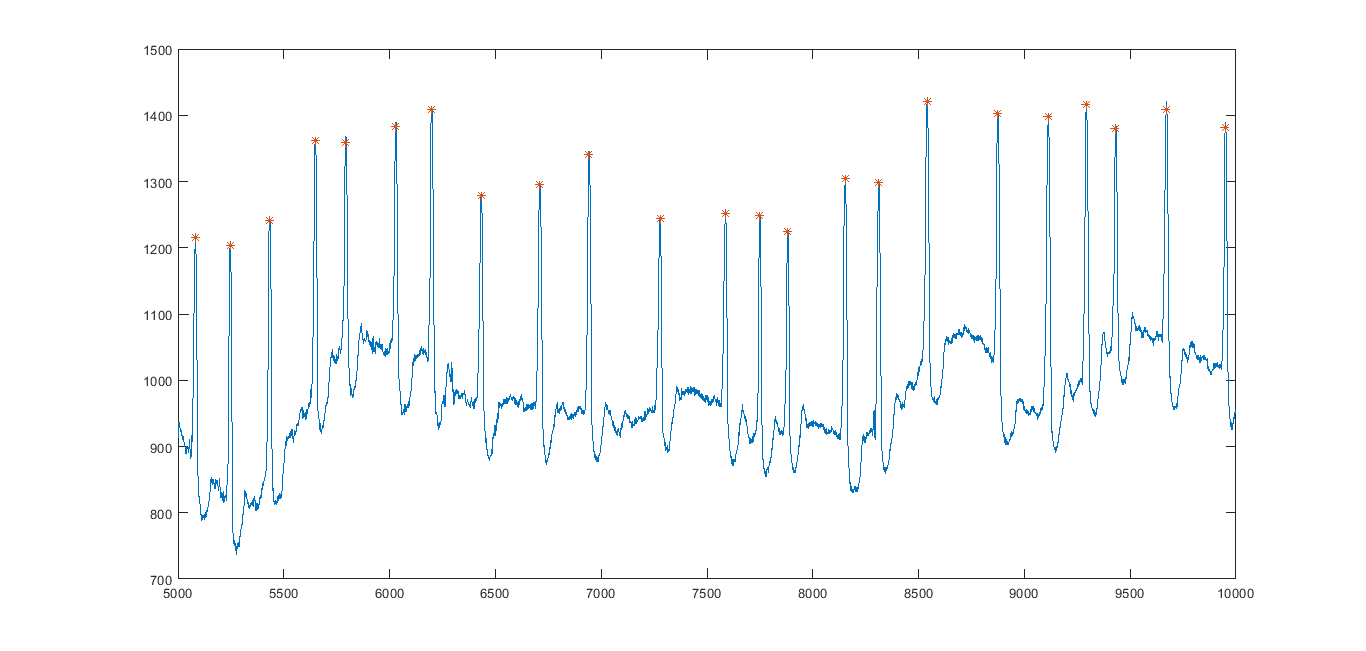
\includegraphics[width=1.4\textwidth,height=10cm]{peaks.png}}\hspace*{-\paperwidth}
\end{figure}


\section{PVC detection}
\subsection{Methods}
Once the R peak of the ECG are detected, three different criterium have been chosen to perform PVC detection: anomalies in peak-to-peak (RR) intervals, QRS area comparison and hermite polynomial analysis.\\
The R-R regularity criterium has the following structure: it first detects the intervals between each couple of peaks, and then computes how much every interval duration is different from the mean duration. The code is the following:
\begin{lstlisting}[caption=RR criterium]
% RR regularity
RRIntervals = zeros(length(ind)-1,1);
for i=2:length(ind)
    RRIntervals(i-1) = ind(i) - ind(i-1);
end
meanRR = mean(RRIntervals);
sdnnRR = calculateSDNNRR(peaks);

myPVCRR = zeros(length(RRIntervals)+1,1);
for i=1:length(RRIntervals)
	myPVCRR(i) = RRIntervals(i) / (meanRR + sdnnRR);
end
\end{lstlisting}

The QRS area criterium makes the computation of the areas below the QRS complexes in the data, and then, like the R-R regularity criterium, compares it with the average area in the acquired data. Specifically the area was computed taking the 0.06 seconds around a peak and calculating the area below the resulting graph via the MATLAB method $trapz()$. This is the code implementing the criterium:
\begin{lstlisting}[caption=QRS area criterium]
% QRS area
area = 0.06;
areaIndex = round(area * fs);

areas = zeros(length(ind),1);
for i=1:length(ind)
    minIndex = ind(i)-areaIndex;
    if minIndex <= 0
        minIndex = 1;
    end
    maxIndex = ind(i)+areaIndex;
    if maxIndex > length(ecg)
        maxIndex = length(ecg);
    end
    actualAreaECG = ecg(minIndex:maxIndex);
    areas(i) = trapz(actualAreaECG);
end

meanArea = mean(areas);

sum = 0;
for i=1:length(areas)
    sum = sum + (areas(i) - meanArea).^2;
end

sdnnArea = sqrt(sum / length(RRIntervals));
myPVCArea = areas(:) / (meanArea + sdnnArea);
\end{lstlisting}

The Hermite criterium makes use of system modeling to consider the data as the output of an ar system. Then, with respect to the location of  the poles of the actual system, if they are out of the (hyper-)circonference of radius 1, which is to say correspond to an unstable system, the considered event corresponds to a PVC occurrence.
In order for the model to work, the peak considered should be necessarily a positive value, so a pre-processing of the peaks has been implemented in order to get coherent data.\\
To get the model for the ar system, the 8 values before and after a peak are taken into account, and so a window of 17 timesteps is obtained. Then, the MATLAB "ar" method is called with a desired order of 2. This has been chosen after considering the perfomances of the criterium with an order ranging from 1 to 8.\\
The roots of the system are found with the MATLAB function "roots()" and then their norm is computed to check if it is greater than 1. Actually, the threshold used is not 1, since after having performed some tests, that would have been too strong and therefore considered every sample as a non-PVC.
Finally, the code is as follows:
\begin{lstlisting}[caption=Hermite criterium]
% hermite
% Code to get positive peaks
for i=1:length(ind)
    if(ind(i)>50 && ind(i)+50<length(ecg))
        start=ind(i)-50;
        finish=ind(i)+50;        
    elseif (ind(i)<50) % case first peak is before 50
        start=1;
        finish=ind(i)+50;
    else % case for last peak
        start=ind(i)-50;
        finish=length(ecg);
    end 
    A=ecg(start:finish); 
    [~,index]=max(A); % find positive peak
    ind(i)=start+index; % code to reassign peak to positive values
end

myPVCHermit = zeros(length(ind),1);
for j=1:length(ind) % Take into account first and last case later
    a=8;
    b=8;
    
    minIndex = ind(j)-a;
    if minIndex <= 0
        minIndex = 1;
    end
    
    maxIndex = ind(j)+b;
    if maxIndex > length(ind)
        maxIndex = length(ind);
    end
    
    window=ecg(minIndex:maxIndex);

    model=ar(window,2);
    A=model.A;
    poles=roots(A);
    tmppvc=0;
    for i=1:length(poles)
        if norm(poles(i))>=0.98
            tmppvc=1;
            break;
        end
    end
    myPVCHermit(j)= tmppvc;
end

\end{lstlisting}

\subsection{Classification}
As it can be noted, while the detection via RR regularities and QRS areas give a "classification" score, a decimal value that quantificates a certain probability of the event being a PVC, the hermite criterium output is a "simple" binary decision between PVC/not PVC. Thus, a specific criterium has to be chosen to combine the different results.
Since the RR regularities or the QRS areas criterium have a really good specificity, if they report a PVC then the global output is set to be a detected PVC: this is why they are OR'd with the third criterium. The third OR case is a AND combination of two criteriums: the combination of RR and QRS scores if they are both quite high but not enough to be greater than 1 by themselves, and a detected PVC from the Hermite criterium. In fact, Hermite criterium has a sensitivity higher than RR+QRS, and as such it eventually compensates combining RR and QRS.
All these considerations have been done after experimental testing on specificity and sensitivity results that can be found in the "Result section".
So, the resulting rule and thresholds are the following:\\\\
$myPVCRR(i) >= 1 || myPVCArea(i) >= 1 || (myPVCArea(i) + myPVCRR(i) >= 1.9) \&\& myPVCHermit(i) == 1$
\\\\

\subsection{Results}

The following table shows the results obtained running the classifier on each patient with five different classification rules: the use of the three "simple" criteriums seen, as well as the combination of RR detection and QRS as well as the total combination of the five of them using the rule described in the last section.
The last row of the table is obtained averaging the values: as it can be seen it gives a good insight over the efficiency of the implemented criteriums: the first three have a really good specificity but low sensitivity, while it's the opposite for the Hermite classifier. Finally, the combination of the three shows a definite and solid increase in both sensitivity and specificity.
\\

\providecommand{\tabularnewline}{\\}
		
\makeatother
\begin{tabular}{|c|c|c|c|c|c|c|c|c|c|c|}
\hline 
 & \multicolumn{2}{c|}{RR} & \multicolumn{2}{c|}{QVC area} & \multicolumn{2}{c|}{RR+QVC} & \multicolumn{2}{c|}{Hermite} & \multicolumn{2}{c|}{Combined}\tabularnewline
\hline 
 & SE & SP & SE & SP & SE & SP & SE & SP & SE & SP\tabularnewline
\hline 
Patient 1 & 0.48 & 0.99 & 0.44 & 0.99 & 0.53 & 0.94 & 0.66 & 0.94 & 0.65 & 0.99\tabularnewline
\hline 
Patient 2 & 0.78 & 1 & 0.95 & 0.98 & 0.97 & 0.99 & 0.68 & 0.91 & 0.99 & 0.98\tabularnewline
\hline 
Patient 3 & 0.85 & 1 & 0.99 & 1 & 0.88 & 1 & 0.27 & 0.93 & 0.99 & 1\tabularnewline
\hline 
Patient 4 & 0.54 & 0.97 & 0.05 & 0.99 & 0.20 & 0.92 & 0.83 & 0.82 & 0.56 & 0.95\tabularnewline
\hline 
Patient 5 & 0.70 & 0.91 & 0 & 0.96 & 0.72 & 0.77 & 0.49 & 0.90 & 0.72 & 0.87\tabularnewline
\hline 
Patient 6 & 0.15 & 0.85 & 0.01 & 0.88 & 0.06 & 0.81 & 0.85 & 0.54 & 0.16 & 0.74\tabularnewline
\hline 
Patient 7 & 0.38 & 0.91 & 0.04 & 0.98 & 0.29 & 0.81 & 0.88 & 0.87 & 0.41 & 0.88\tabularnewline
\hline 
Patient 8 & 0.33 & 0.90 & 0.94 & 1 & 0.72 & 0.87 & 0.36 & 0.97 & 0.96 & 0.90\tabularnewline
\hline 
Patient 9 & 0.51 & 0.99 & 0.18 & 0.97 & 0.47 & 0.91 & 0.86 & 0.91 & 0.64 & 0.95\tabularnewline
\hline 
Patient 10 & 0.70 & 0.99 & 0.77 & 0.99 & 0.80 & 0.98 & 0.94 & 0.32 & 0.97 & 0.98\tabularnewline
\hline 
Patient 11 & 0.65 & 1 & 0.01 & 0.98 & 0.16 & 1 & 0.92 & 0.13 & 0.70 & 0.98\tabularnewline
\hline 
Average & 0.55 & 0.96 & 0.40 & 0.97 & 0.53 & 0.91 & 0.70 & 0.75 & 0.70 & 0.93\tabularnewline
\hline 
\end{tabular}

\hfill \break
A visual rapresentation of the performances can be seen in the following graph, where each bar is the result for a patient, while "clusters" of bars are representative of a criterium/metric.

\begin{figure}[h!]

\hspace*{-\dimexpr\oddsidemargin+1in\relax}\makebox[\paperwidth]{%
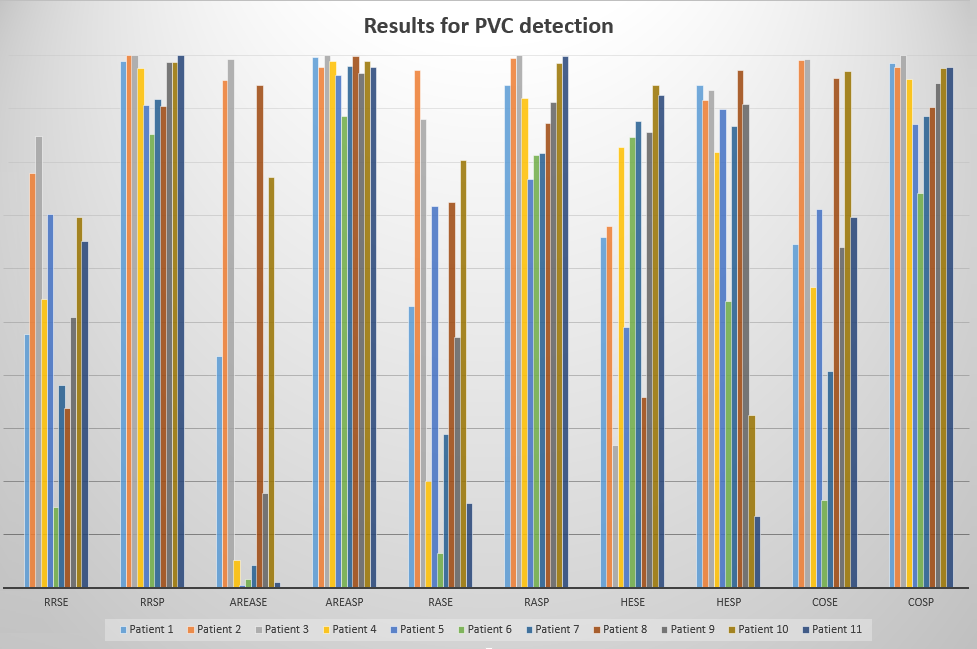
\includegraphics[width=1.4\textwidth,height=12cm]{resultsPVC.png}}\hspace*{-\paperwidth}
\end{figure}

\clearpage


\section{AF}
Atrial fibrillation, rather than an actual istantaneous occurence of an event, is a condition that affects interval of times of a patient.
Because of this, every analysis is performed after windowing the signal: thus every window is recognized as being an occurence of AF or not. Subsequently, the single timestep belonging to a window are classified as 0s or 1s following the window classification.
The implemented code takes into account windows of size 20.
For AF detection, two different criterium have been used: irregularities in the R-R intervals and power content of the ecg spectrum.
\subsection{Methods}
\subsubsection{R-R regularity}
- RR intervals: same as for PVC just for all the different windows, than we compare the window values and try to get smart assumptions

\subsubsection{LF/HF ratio}
The second criterium chosen to find an atrial fibrillation works with the power content of the signal's frequences: since a fibrillation is characterized by the presence of noise in the ECG data, this can be easily detected in the frequency domain.
In fact, a "regular" heart rate spectrum has most of its power in the low part of the spectrum, which considering a usual ecg signal is the range of frequencies  before and around 40Hz.
However, before of actually analizying the spectrum, since the QRS complex carries significant components in higher frequencis, the signal has to be "cleaned", removing the actual QRS part.
In order to do so, given a peak, this code chooses the time steps right before and after the peak and "cleans" the data:

\begin{lstlisting}
front = 0.06;
frontIndex = front * fs;
back = 0.02;
backIndex = back * fs;
for j=1:length(tempPeaks)
	minIndex = tempPeaks(j)-frontIndex;
	maxIndex = tempPeaks(j)+backIndex;
	if minIndex < 1
		minIndex = 1;
	end
	if maxIndex > length(tempEcg)
		maxIndex = length(tempEcg);
	end

	for k=minIndex:maxIndex
		tempEcg(k) = NaN;
	end
end
tempEcg(isnan(tempEcg)) = [];
\end{lstlisting}

After this, the power information is retrieved using MATLAB's function bandpower(). Then the ratio is stored to actually detect an AF occurrence. If the ratio is lower than a certain threshold (chosen after testing various configurations, as it will be shown), it means that the higher frequencies (in this case from 40 to 125, nyquist frequence) retain more power than usual and that the ecg has "noise" associated to fibrillation.

\begin{lstlisting}
LF = bandpower(tempEcg, fs, [0 40]);
HF = bandpower(tempEcg, fs, [40 124]);
LFHF = LF / HF;
lfhfWindows(index) = LFHF;
\end{lstlisting}


\subsection{Classification}
The RR criterium requires setting the threshold (...) 
%TODO How did we set the 0.9?

In order to set the threshold for the LF/HF ratio criterium as well as to test the best combination, a series of experimentation have been done with the dataset and the performance of the different criteriums was obtained.
The two criteriums were combined using an and rule:
\\$sdnnRRWindows(i) < thresholdRR \&\& lfhfWindows(i) < tresholdLFHF$\\
The results of the testing are reported in the following table: for each criterium the left column is sensitivity, and the right one is specificity.

\begin{table}[htbp]
  \centering
  \caption{Parameter tuning}
    \begin{tabular}{c |rr|rr|rr|}
    \multicolumn{1}{c|}{Threshold} & \multicolumn{2}{c|}{RR regularity} & \multicolumn{2}{c|}{LF/HF ratio} & \multicolumn{2}{c|}{Combination} \\ \hline
    0,4   & 1     & 0,431257 & 0,732699 & 0,346755 & 0,732699 & 0,571755 \\
    0,5   & 1     & 0,431257 & 0,893313 & 0,280466 & 0,893313 & 0,547132 \\
    0,6   & 1     & 0,431257 & 0,954536 & 0,229618 & 0,954536 & 0,505544 \\
    \end{tabular}%
  \label{tab:addlabel}%
\end{table}%

The threshold setting does not influence the R-R regularity criterium, but in the LF/HF ratio it has a strong influence on the sensitivity and specificity. Making it higher means that more samples are classified as AF, actually improving sensitivity at the cost of a loss of specificity.
Both criteriums alone have a really good sensitivity while poor specificity, which is to say the are too shallow in classifying samples as AF occurences. The combination of the two attempts to cope with this and therefore shows significant improvement on the specificity, performing better than both criteriums alone. However it is to be noted that being it an AND, combining the values bounds the sensitivity to the lowest possible, specifically the LF/HF criterium.
As it can be seen, the best values are obtained with the combination of the two methods, when the threshold for the LF/HF ratio is set to 0.6.  Given the premises, this threshold allows the best tradeoff for sensitivity gain/specificity loss, with combination performing better than the other two criteriums.

\subsection{Results}

% Table generated by Excel2LaTeX from sheet 'Foglio2'
\begin{table}[htbp]
  \centering
  \caption{Add caption}
    \begin{tabular}{rrrrrr}
    1     & 0,997183 & 0,954476 & 0     & 0,954476 & 0,997183 \\
    1     & 0,87055 & 0,419718 & 0,87055 & 0,419718 & 0,87055 \\
    1     & 0,5   & 1     & 0,083333 & 1     & 0,583333 \\
    1     & 0,323667 & 0,854736 & 0     & 0,854736 & 0,323667 \\
    1     & 0,666667 & 1     & 0,23825 & 1     & 0,73825 \\
    1     & 0,666667 & 1     & 0,716117 & 1     & 0,882783 \\
    1     & 0,75875 & 1     & 0,592083 & 1     & 0,842083 \\
    1     & 0,166667 & 1     & 0,166667 & 1     & 0,25 \\
    1     & 0,166667 & 1     & 0,023533 & 1     & 0,1902 \\
    1     & 0,083333 & 1     & 0,166667 & 1     & 0,25 \\
    1     & 0,76415 & 1     & 0,25  & 1     & 0,76415 \\
    1     & 0,73465 & 1     & 0,083333 & 1     & 0,817983 \\
    1     & 0,25  & 1     & 0,083333 & 1     & 0,25 \\
    1     & 0,73035 & 1     & 0,25  & 1     & 0,73035 \\
    1     & 0     & 1     & 0,083333 & 1     & 0,083333 \\
    1     & 0     & 1     & 0,192583 & 1     & 0,192583 \\
    1     & 0,083333 & 1     & 0,25  & 1     & 0,25 \\
    1     & 0     & 0,952713 & 0,083333 & 0,952713 & 0,083333 \\
    1     & 0,431257 & 0,954536 & 0,229618 & 0,954536 & 0,505544 \\
    \end{tabular}%
  \label{tab:addlabel}%
\end{table}%



\section{Conclusions}

\subsection{PVC}
MUITO BEM!!!

\subsection{AF}
0.5 * muito bem!

\end{document}
